%----------------------------------------------------------------------------------------
%	PACKAGES AND DOCUMENT CONFIGURATIONS
%----------------------------------------------------------------------------------------

\documentclass{article}

\usepackage[numbers]{natbib}
\usepackage{graphicx} % Required for the inclusion of images
\usepackage{natbib} % Required to change bibliography style to APA
\usepackage{amsmath} % Required for some math elements

\usepackage{geometry}
\usepackage{lmodern}
\usepackage{hyperref}
\usepackage{fontspec}
\usepackage{titling}
\setlength\parindent{0pt} % Removes all indentation from paragraphs


\renewcommand{\labelenumi}{\alph{enumi}.} % Make numbering in the enumerate environment by letter rather than number (e.g. section 6)

%\usepackage{times} % Uncomment to use the Times New Roman font

%----------------------------------------------------------------------------------------
%	DOCUMENT INFORMATION
%----------------------------------------------------------------------------------------

 % Title


\begin{document}

\author{
  Fuchs, Max\\
  \texttt{2908207}
  \and
  Gärtner, Christoph (Group AD)\\
  \texttt{2766889}
  \and
  Hofmann, Tobias\\
  \texttt{2350059}
  \and
  Kalabić, Edin\\
  \texttt{2401115}
  \and
  Linke, Alexander\\
  \texttt{2274630}
}

\pretitle{%
  \begin{center}
  \LARGE
  
\includegraphics[width=9cm]{img/logo_schriftzug.png}\\[\bigskipamount]
}
\posttitle{\end{center}}

\title{TK3: Ubiquitous / Mobile Computing}



\maketitle

%----------------------------------------------------------------------------------------
%	SECTION 1
%----------------------------------------------------------------------------------------
% Include instructions or scripts to execute the project
% uploaded a short demonstration video (make it fancy)
% Provide a short, but precise, documentation


\section{Introduction}

% Introduction


The gain in polularity of artifical intelligence in the recent years motivated our decision to build a smart lamp -- with machine learning as driving actor. The lamp ought to be smart enough to toggle itself \textbf{on} and \textbf{off}, solely based on data. Data which is collected at the beginning, in the so-called \emph{training-phase}, by manual user interaction with a physical switch.

Our concise two minute video (\url{https://www.youtube.com/watch?v=AOq6Cx7RbSw}) will give a short visual overview of the project.


\subsection{Hardware}

To keep monetary costs as low as possible, we tried using only the available hardware of prior excercises, i. e. a Raspberry Pi, several ESP32 developement boards and a broad range of available sensors+actors. But to avoid having to deal with mains electricity, because we as computer scientists should not act on exposed 230V wires with superficial knowledge, we were given three \emph{Phlips Hue}\footnote{\url{http://www2.meethue.com/de-DE}} lamps with a network bridge for control.

\subsection{Theoretical Layout}

The Raspberry Pi ended up as the projects control center. All sensory data, as well as onboard metrics like \emph{time of day} and \emph{daylight} are flowing to the Pi, where it is logged during the training-phase. The training-phase is exactly one week after first start-up or after initating a reset. After training-phase, the Raspberry Pi would query the trained model continuously with current sensor values, to decide wether to turn the lamp on or off.

Because the Pi is very limited in regards to RAM and processing power, we couldn't use a machine learning technique like deep neural networks to train the model. Whereas only classification would be possible. But because the model also had to be learned on the Pi itself, we moved away from the idea of a neural network and towards a decision tree.

Unlike a neural network, a decision tree requires discrete values, which forced us to lessen resolution of continuous values like \emph{time of day}. 

Following is the complete list of used metrics and their resolutions:

\begin{itemize}
    \item Time of Day
         \begin{itemize}
           \item Early Morning
           \item Morning
           \item Early Afternoon
           \item Late Afternoon
           \item Night
        \end{itemize}      
    \item Daylight
        \begin{itemize}
           \item True / False
        \end{itemize}    
    \item Weekday
     \begin{itemize}
           \item Mo -- So
        \end{itemize}   
    \item One entry per networked device
       \begin{itemize}
           \item Device Status (Connected, Disconnected)
          \end{itemize}
    \item Lamp Status
         \begin{itemize}
           \item On / Off
        \end{itemize}   
\end{itemize}

\begin{figure}
  \centering
    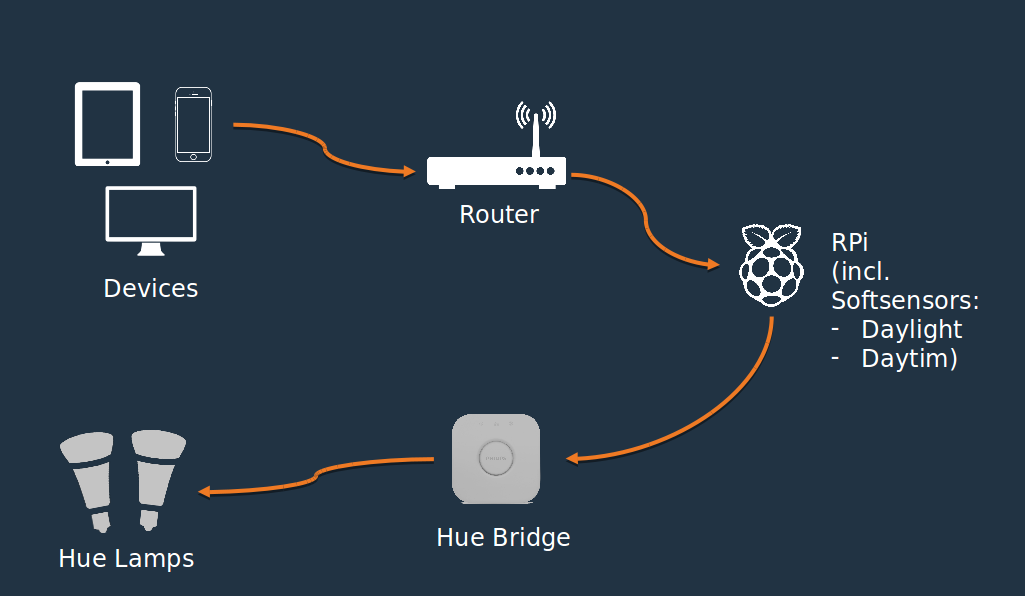
\includegraphics[width=1.0\textwidth]{../../ArchitectureFinal.png}
  \caption{Architecture}
  \label{fig:architecture}
\end{figure}


\section{Instructions for Code Execution}

% Instructions

Get a MQTT Broker running in your network (e.g. on the Raspberry Pi). Adjust the IP Adress (192.168.1.226) in RaspberryPi/DataCollector.py and Linksys\_Router/publish\_wifi\_clients.py to match the ip of the client that is running your MQTT broker.

Get yourself a Linksys WRT1900AC Router with openWRT operating system. The router needs to be in a network with the MQTT Broker and should be configured as an Access Point on your WLAN Devices. Edit the devices Dictionary in Linksys\_Router/publish\_wifi\_clients.py to match your personal Wifi devices and respective MAC-Addresses. Install Python, pip and the paho library on the router. Run the Linksys\_Router/publish\_wifi\_clients.py script on the Router.

Set up a phillips HUE in your network. Adjust RaspberryPI/LampControl.py to match your Hue's ip address.

Copy the RaspberryPI folder to your Raspberry Pi and run the DataCollector Script. This will store information about your lamps current status, daytime, connected devices, etc. in 'decision\_tree\_data' and 'raw' files. Let the data collection run for a few weeks.

After collecting data, run the RaspberryPi/ModelTrainer.py on your Raspberry. It will build a decision tree model based on the collected data stored in decision\_tree\_data.

Once the model is trained you can run RaspberryPI/Evaluator.py on your Raspberry. This script will switch the Hue on and off according to the decision tree model.
 \label{section:2}

\section{Implementation}

Our code is completely written in Python. Python allows us to quickly test and generate functioning examples. Also many machine learning libraries provide excellent Python APIs, such as the libraries we used in the implementation.

Our Code is structured in two main logic parts, consisting of several smaller, partly shared, modules and classes.


\subsection{Training Phase}

The class \emph{DataColletor} can be queried for the most recent sensor data. \emph{DataColletor} internally listens for MQTT events and caches the latest value. At query time, all MQTT values are augmented with computed properties like time of day, status of the lamp, or daylight.

\emph{DataWriter.py} is responsible to store the training data at a pre-defined interval, by querying \emph{DataColletor}. The query-result is simply appended in a text file.

After the collection phase, the decision tree is computed. It gives us insight in when to turn the lamp on or off. This tree is computed in \emph{ModelTrainer.py}.

\subsection{Evaluation Phase}

When the model is sucessfully created, it is evaluated. This is also done, just like the data collection, in a pre-defined interval. \emph{Evaluator.py} gets the current sensor values, by quering \emph{DataColletor} and with them as input, in turn queries the prior computed decision tree model. The decision tree query now results in wether the lamp should be turned on or off. The class \emph{LampControl} provides an interface for doing just that.

\emph{LampControl} sends API requests via HTTP to the \emph{Philips Hue Bridge}.

\section{Conclusion and Outlook}


Due to the very short time we had to complete this project, we couldn't collect as much training data as we wanted. Partly also because of problems with the Raspberry Pi's timezone setting over Ethernet. Our final tree reflects just that constrained enviroment. Despite only turning the lights on at 2 distinct junctions, the tree still achieves a 91\% accuracy on the trained data.

\begin{figure}
  \centering
    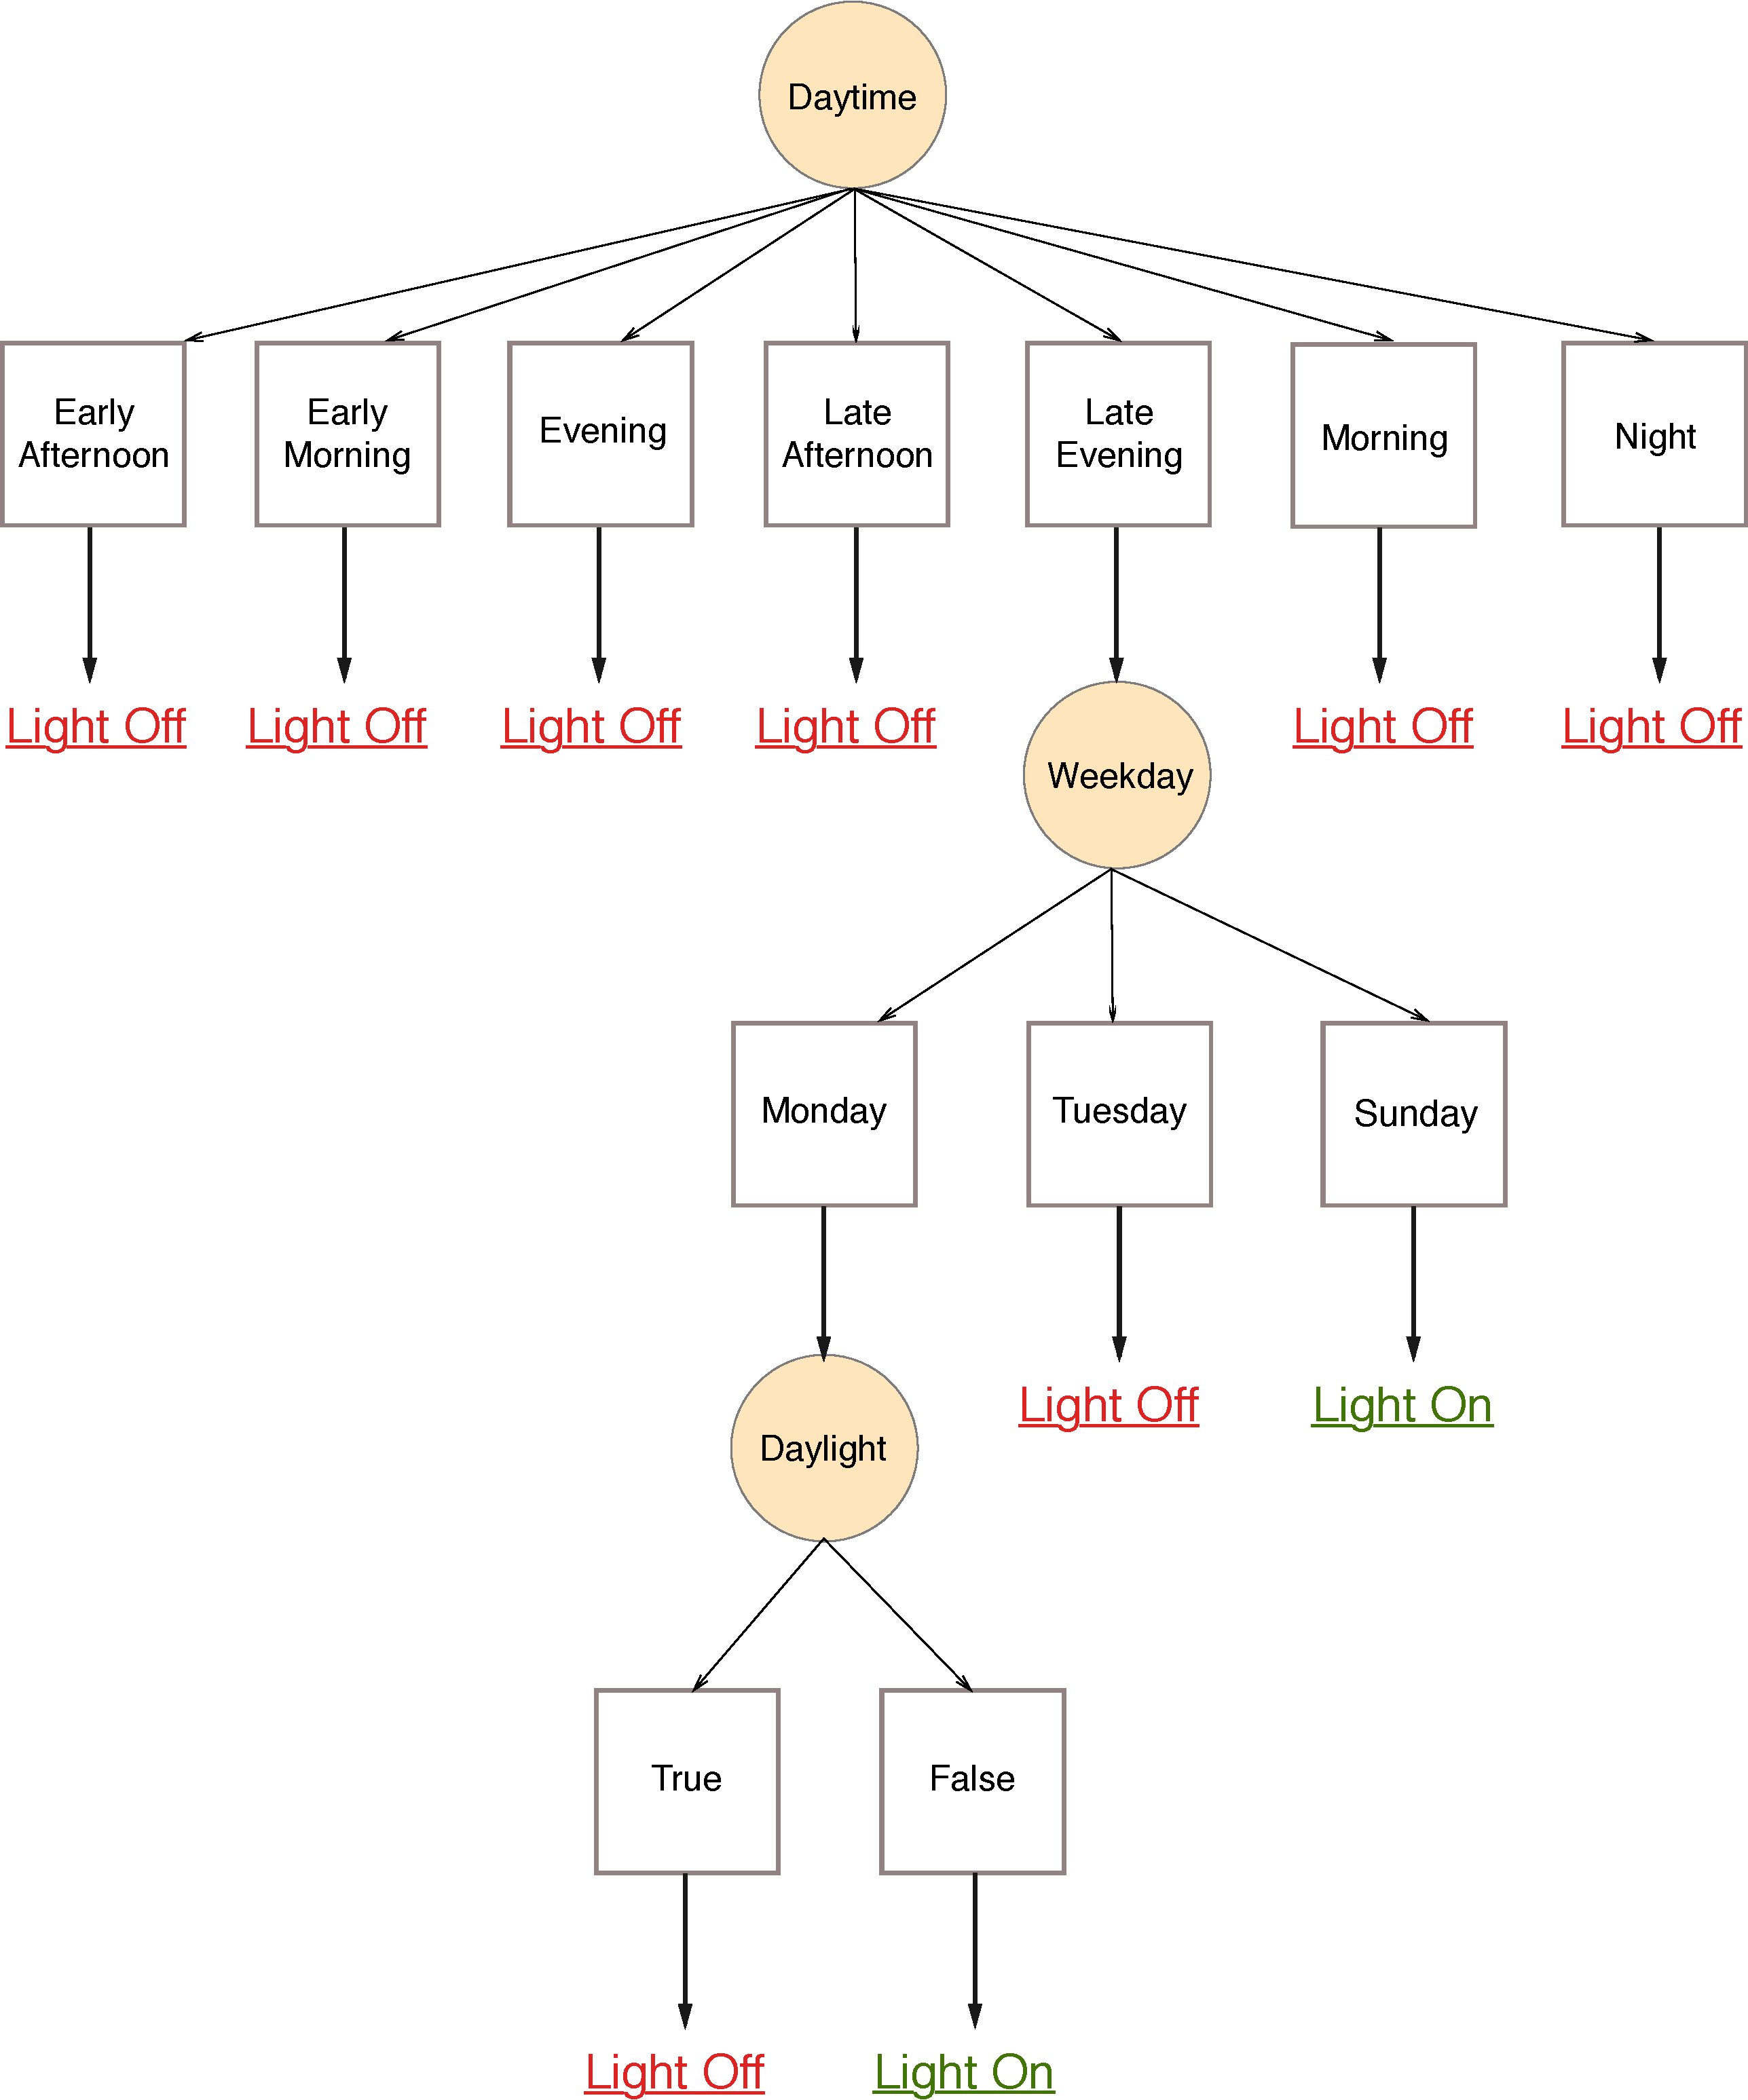
\includegraphics[width=1.0\textwidth]{img/tree.pdf}
  \caption{Resulting decision tree}
  \label{fig:result}
\end{figure}

Interesting would be a result with complete full week long training.

\subsection{Future Work}

Future work could improve the SMART Machine Learning Lamp in the following ways.

The lamps underlying decision tree model currently cannot be easily adjusted after the initial training, without a complete new training-phase. Future work could improve upon that, and continuously improve the model with the help of ongoing user interaction with the lamp. This also includes when new devices that should impact the decision are brought to the household.






\chapter*{Resposibilities}

\begin{itemize}
\item Logo / Video: Alexander Linke, Edin Kalabić
\item Presentation: Tobias Hofmann, Alexander Linke, Max Fuchs
\item Documentation: All
\item Lamp Control: Alexander Linke, Edin Kalabić
\item Softsensor Daylight: Alex, Max Fuchs, Edin Kalabić
\item Softsensor Wifi-Devices: Max Fuchs
\item Evaluator: Christoph Gärtner, Max Fuchs
\item Decision Tree Model Trainer: Max Fuchs
\item Data Collection: Christoph Gärtner, Max Fuchs
\item Class structure: Christoph Gärtner
\end{itemize}





%----------------------------------------------------------------------------------------
%	BIBLIOGRAPHY
%----------------------------------------------------------------------------------------

\bibliographystyle{apalike}

\bibliography{sample}

%----------------------------------------------------------------------------------------


\end{document}
